%Review of existing harmonic excitation.
%	Nonlinear Systems
%		Traditional Metrics (THD, IMD)
%		Minimisation of Nonlinear Distortion
%		Advent of "Nonlinear Niceness"
%	Timbre of nonlinear distortions (Martens and Marui type shit)
%	Uses of Harmonic Excitation
%	Harmonic Generation Methods
%		Static Nonlinearities
%		Bandwidth Extension (high frequency reconstruction)
%		Individual Harmonic Generation (SMC paper)
%		Psychoacoustic Enhancers

\chapter{Evaluation of Harmonic Excitation Algorithms}
\label{chap:ExcitationEvaluation}

\section{Evaluation Criteria for Assessing Harmonic Excitation Methods} % section name not very clear
\label{sec:ExcitationEvaluation-Evaluation}
	Harmonic excitation algorithms developed for the applications discussed in the Section
	\ref{sec:Excitation-Uses} are specialised to perform a particular task. As this work is concerned with
	the application of harmonic excitation to real time timbral control some algorithms in the literature may
	not be applicable. In this section a set of criteria for assessing the suitability of a harmonic excitation
	algorithms for use in this work are suggested.  These criteria are then used to asses various algorithms in Section
	\ref{sec:ExcitationEvaluation-Comparison}. 

	To prove useful for real time timbral control a harmonic excitation algorithm should provide efficient, intuitive
	control over where energy is introduced to a signal. This behaviour can be split into the following areas:

	\begin{itemize}
		\item Low Complexity.
		\item Homogeneity
		\item Spectral Characteristics.
		\item Temporal Characteristics.
		\item Flexibility.
%		\item Naturalness.
	\end{itemize}

	The following sections will discuss what behaviour is desirable in these areas.

	\subsection{Complexity}
	\label{sec:ExcitationEvaluation-Evaluation-Complexity}
		Audio effects are typically required to operate in real time. This speeds up music production as effect
		parameters can be adjusted while audio is playing and the results heard immediately. In order to achieve
		this, effects must process audio with minimal latency. 

		In order to ease the computational load on the processor, audio processing if often done in blocks. A
		certain number of samples are recorded into a buffer and then all processed at once. This introduces some
		latency into the system, the processing buffer must be filled with samples from the input before an output
		can be produced. The larger the processing buffer size the more latency but the less the computational load
		as the cost of constructing and moving buffers is amortised across a greater number of samples. Any
		processing applied to the block of audio must be completed within the allowed latency time, if not there
		will be gaps between blocks during playback causing audible anomalies.

		For real time audio effects it is crucial to keep throughput latency to a minimum. \citet{lester2007the}
		suggest that, depending on the scenario, latencies as small as 1.4ms could be deemed unacceptable. In order
		to keep latency to a minimum, processing algorithms should be able to run in real time when using a small
		buffer size.

	\subsection{Homogeneity}
	\label{sec:ExcitationEvaluation-Evaluation-Homogeneity}
		In order to be intuitive an audio effect it should produce a similar perceptual effect across a wide range
		of input signals. Often this is not the case with traditional audio signal processing methods. Take the EQ
		for example. We can set up an EQ to boost some frequencies in a desired range. The spectra of signals with
		energy in this frequency range will be altered while those of signals with no energy in that band will be
		unaffected. This problem is compounded when the effect being applied is non-homogeneous.
		
		Nonlinear systems are typically non-homogeneous. This is undesirable when using them to achieve timbral
		control as it means the effects are less easy to predict. Different timbral transforms could be applied to
		the same signal if its amplitude is changed slightly. From a user's point of view this makes control of the
		system less intuitive as control parameters can change function depending on signal level.

	\subsection{Spectral Characteristics}
	\label{sec:ExcitationEvaluation-Evaluation-SpectralCharacteristics}
		All the algorithms presented in this Section \ref{sec:Excitation-Methods} introduce new spectral content to
		a signal. Depending on the algorithm wide bands of energy or individual harmonics can be excited. For
		intuitive timbral control it is desirable that these spectral effects are similar across a wide range of
		input signals. For example a system designed to only generate harmonic partials should not introduce
		inharmonicity for any input signal.

	\subsection{Temporal Characteristics}
	\label{sec:ExcitationEvaluation-Evaluation-TemporalCharacteristics}
		\citet{larsen2004audio} discuss the temporal effects of several bandwidth extension algorithms. Their
		primary concern however is ensuring that as little alteration is made to the temporal envelope of a signal
		as possible. For timbral manipulation it is not necessary to be this restrictive. As discussed in Section
		\ref{sec:Timbre-LowLevelFeatures} one of the properties of a signal which contributes to its timbre is how
		it evolves over time. As with other aspects of excitation algorithms it is more important that the temporal
		characteristics are predictable and consistent across a wide range of signals.

	\subsection{Flexibility}
	\label{sec:ExcitationEvaluation-Evaluation-Flexibility}
		Each excitation method allows for different amounts of control over the spectral content introduced. Finer
		control of this allows a method to be used in a wider range of situations. The flexibility of a method
		describes how well it can be adapted for different processing needs and how applicable it is across a wide
		range of input signals.

\begin{landscape}
\section{Comparison Summary}
\label{sec:ExcitationEvaluation-Summary}

	\begin{table}[h!]
		\centering
		\begin{tabular}{|c|c|c|c|c|c|c|}
			\hline
			\bf{Method} & \bf{Complexity} & \bf{Homogeneity} & \bf{Spectral Properties} & 
		 	\bf{Temporal Properties} & \bf{IMD} & \bf{Flexibility} \tabularnewline % & \bf{Naturalness}
			\hline
			\hline
			Static Nonlinearity & $\mathcal{O}(n)$ & & & & & \tabularnewline
			\hline
			Rectifier & $\mathcal{O}(n)$ & & & & & \tabularnewline
			\hline
			Integrator & $\mathcal{O}(n)$ & & & & & \tabularnewline
			\hline
			Multiplier & $\mathcal{O}(n)$ & & & & & \tabularnewline
			\hline
			SSBA & $\mathcal{O}(n)$ & & & & & \tabularnewline
			\hline
			IAP & $\mathcal{O}(n)$ & & & & & \tabularnewline
			\hline
			Spectral Replicator & $\mathcal{O}(n)$ & & & & & \tabularnewline
			\hline
			Spectral Mirror & $\mathcal{O}(n)$ & & & & & \tabularnewline
			\hline
			Spectral Stretch & $\mathcal{O}(n\log{n})$ Assuming FFT used & & & & & \tabularnewline
			\hline
		\end{tabular}
		\caption{A summary of the comparison of excitation methods.}
		\label{tab:ComparisonSummary}
	\end{table}

\end{landscape}

\section{Method Comparison}
\label{sec:ExcitationEvaluation-Comparison}
	In the section the algorithms discussed in Section \ref{sec:Excitation-Methods} are evaluated against the criteria
	given in Section \ref{sec:ExcitationEvaluation-Evaluation}. Techniques for improving performance with regard to
	particular criteria are suggested and discussed. 

	\subsection{Complexity}
	\label{sec:ExcitationEvaluation-Comparison-Complexity}
		The algorithms with the lowest complexity are the static nonlinearities. The application of a static
		nonlinearity involves only a few simple operations for each input sample. Perhaps the simplest case is that
		of full wave rectification in which a single absolute value operation is applied for each sample. As the
		characteristic curve of the nonlinearity becomes more complex the computational load increases. Hard
		clipping and half wave rectification require comparison operations to determine which samples should be
		altered. 

		Further complexity is introduced where the characteristic curve require some computation such as with
		exponential distortion and soft clipping. The transition section of the soft clipper given in Equation
		\ref{eq:SymmetricSoftClipping} requires a considerable number of operations to calculate. In situations
		where the number of calculations becomes to large the computational load can be decrease using a
		precomputed lookup table in input and output values.

		As static nonlinearities process each sample individually, the amount of work required per unit time of
		audio grows linearly with the sampling rate.

		Every other algorithm presented in Section \ref{sec:Excitation-Methods} involves some dependence on the
		previous input and output samples of the system. Implementing these algorithms involves the use of
		additional memory.

		The simplest algorithm which requires this additional memory is the integrator given in Equation
		\ref{eq:Integrator}. The previous input sample is needed in order to detect zero crossings in the input and
		the previous output sample is needed to apply the integration. The amount computation performed for this
		system is comparable to that of a simple static nonlinearity, giving a very low computational load.

		Spectral folding using Equation \ref{eq:SpectralFolding} require a low pass filter in order to reduce
		aliasing. This filter comprises the majority of the complexity of the system leading to a trade off between
		computational complexity and the level of aliasing. Increasing the order of the filter will better reduce
		aliasing while increasing the overall complexity.

		More complex filtering is required by those algorithms which operate on an analytic signal. The Hilbert
		transform of the input signal must be computed in order to construct the analytic signal. The Hilbert
		transform filter used must have a suitably consistent response for a wide range of frequencies so the
		resulting harmonic excitation gives similar results at different frequencies.

		A high order FIR Hilbert transform filter is required to give a suitably flat magnitude response. As the
		order of this filter is increased the computation time rises along with the amount of delay needed to make
		the filter causal. A lower complexity IIR phase splitter can be used in order to reduce the computational
		load. The implementation given by \citet{niemitalo2003hilbert} consists of eight biquad filters and a one
		sample delay. This provides a reasonable compromise between accuracy, complexity and introduced delay.

		Once an analytic signal has been constructed, little additional computation is required. SSBA requires the
		evaluation of a complex exponential for each sample. IAP and spectral replication, however, require the
		computation of trigonometric functions, be it to calculate the complex argument of the analytic signal or to
		synthesis a modulating signal.

		Spectral stretching using a phase vocoder requires a large amount of computation. Calculating the STFT
		involves splitting the signal into frames on which the DFT is then computed. The phase correction for each
		frame must then be computed and applied before the inverse DFT of each frame is taken and the frames summed
		back together. The resulting signal then needs to be resampled requiring further operations. If the scaling
		factor is not an integer value, the resampling process will require additional interpolation calculations.
	
		Several steps can be taken to reduce the work needed when using a phase vocoder. The computational
		complexity of the DFT calculations can be reduced by using the fast Fourier transform
		\citep{portnoff1976implementation}. When shifting the frequencies upwards, the amount of work can be further
		reduced by resampling the signal before calculating the STFT \citep{laroche1999new}. This way there are
		fewer frames for which the DFT need be calculated.

		The computational complexity of STTR depends on the ratio of the step size, $R$, and the length of the
		window function $L$ in samples. As $\frac{R}{L}$ decreases the number of overlapping frames needed to
		calculate an output sample increases, increasing the computational load. Time reversal of the frames
		introduces an $L$ sample delay to the signal as the samples at the end of the first frame are needed to form
		the start of the signal.

	\subsection{Homogeneity}
	\label{sec:ExcitationEvaluation-Comparison-Homogeneity}

		\subsubsection*{Static Nonlinearities}
			The homogeneity of a static nonlinearity depends on the nonlinear function used. For different
			input amplitudes the set of harmonics generated by a given static nonlinearity will change. The
			ways in which this set of harmonics changes was investigated by \citet{enderby2012harmonic}.

			In that study the effects of several soft clippers on sinusoidal inputs were analysed. The levels
			of individual harmonics are plotted as a function of input amplitude. Figures
			\ref{fig:HardClippingHarmonics} and \ref{fig:SoftClippingHarmonics} show these plots for the
			clipping functions described previously.

			\begin{figure}[h!]
				\centering
				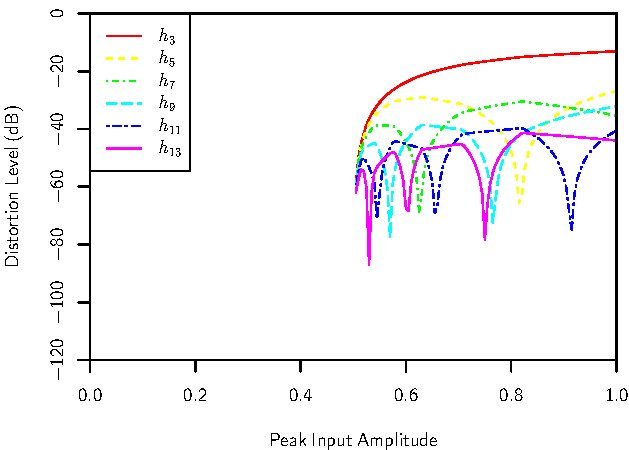
\includegraphics{chapter5/Images/HardClippingHarmonics.pdf}
				\caption{Individual harmonic distortion levels for Equation \ref{eq:SymmetricHardClipping}
					 with a threshold of 0.5.}
				\label{fig:HardClippingHarmonics}
			\end{figure}

			\begin{figure}[h!]
				\centering
				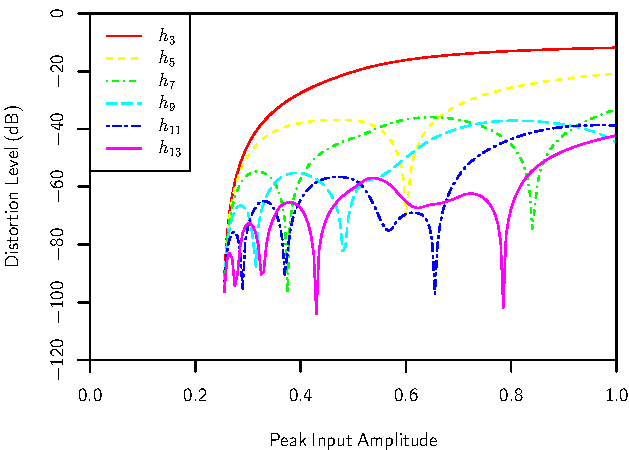
\includegraphics{chapter5/Images/SoftClippingHarmonics.pdf}
				\caption{Individual harmonic distortion levels for Equation \ref{eq:SymmetricSoftClipping}
					 with a threshold of 0.5.}
				\label{fig:SoftClippingHarmonics}
			\end{figure}

			The first thing to note is that new harmonic components are only introduced once the input
			amplitude extends out of the linear section of the characteristic curve. Once input amplitude
			reaches a sufficient level harmonics are introduced but their amplitudes all vary independently.

			This behaviour can be improved on through the use of a different clipping function. Equation
			\ref{eq:SymmetricExponentialClipping} shows a function used to apply exponential clipping to a
			signal.
			
			\begin{equation}
				y[n] = \begin{cases}
					t\sgn(x[n]) & \text{if $\abs{x[n]} > t$} \\
					t\sgn(x[n]) \left(1 - \abs{\frac{x[n]}{t} - \sgn(x[n])}^{E} \right) &
						\text{otherwise}
				\end{cases}, \quad t \geq 0 \ \text{and} \ E > 1
				\label{eq:SymmetricExponentialClipping}
			\end{equation}

			Where $E$ is a second parameter called the exponent. One advantage of this clipper is that it has
			no linear section. This means that harmonics are generated for input signals of any amplitude.
			Another advantage is that the levels of the generated harmonics vary more uniformly with input
			amplitude as shown in Figure \ref{fig:ExponentialClippingHarmonics}.

			\begin{figure}[h!]
				\centering
				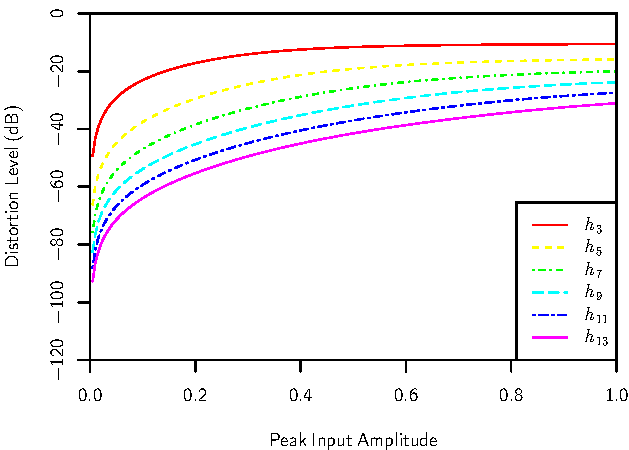
\includegraphics{chapter5/Images/ExponentialClippingHarmonics.pdf}
				\caption{Individual harmonic distortion levels for Equation
					 \ref{eq:SymmetricExponentialClipping} with a threshold of 0.5 and an 
				         exponent of 5.}
				\label{fig:ExponentialClippingHarmonics}
			\end{figure}

			The non-homogeneity of simple clipping systems can be counteracted by introducing gain stages
			either side of the clipping stage. The first gain stage scales the signal so that the clipping
			stage will always clip the same proportion of the signal. The second gain stage scales the signal
			back to the original input amplitude. Analogously the clipping function can be scaled so it
			always clips the same proportion of the signal, as done by \citet{deman2014adaptive}.

		\subsubsection*{Rectification}
			One of the main advantages of rectifiers is that they are exhibit positive homogeneity (they
			satisfy Equation \ref{eq:homogeneity} only for non-negative values of $a$). For full wave
			rectification this can be summarised using Equation \ref{eq:FullWaveRectificationHomogeneity}.

			\begin{equation}
				\abs{ax[n]} = a\abs{x[n]}, \quad \forall a \in \textbf{R}_{\geq 0}
				\label{eq:FullWaveRectificationHomogeneity}
			\end{equation}

			Half wave rectification is not homogeneous for negative values of $a$ as the negative portions of
			the input signal are zeroed. If a negative gain is applied prior to this process, what were the
			positive portions of the input signal will be zeroed.

		\subsubsection*{Integrator}
			Integration is a homogeneous operation. This is an advantage over certain static nonlinearities as
			though more operations are needed per sample no further work is needed to make the system
			homogeneous. If a homogeneous system is required, it may be more efficient to use an integrator
			over a static nonlinearity.
		
			\note
			{
				Formal proof?
			}

		\subsubsection*{Multiplier}
			Exponentiation is a non-homogeneous operation. Any amplitude applied to a signal before processing
			is also raised to the exponent, as shown in Equation \ref{eq:MultiplierHomogeneity}.

			\begin{equation}
				(ax[n])^{h} = a^{h}x[n]^{h}
				\label{eq:MultiplierHomogeneity}
			\end{equation}

			Unlike clippers there is no threshold parameter to change in response to the amplitude of the input
			signal. Gain stages can be added before and after the nonlinearity in order to make the system's
			response to different input amplitudes more uniform.

		\subsubsection*{SSBA}
			As with multipliers, SSBA is a non-homogeneous process. The amplitude envelope of the $h$\super{th}
			order automodulation is the amplitude envelope of the original signal raised to the power $h$. 

		\subsubsection*{IAP}
			In the IAP method the magnitude and phase information of a signal are separated. The phase
			information is scaled in order to increase the frequency while the magnitude information is left
			unaltered. This preservation of magnitude information mean that the IAP method is a homogeneous
			system.

			\note
			{
				Formal proof?
			}

		\subsubsection*{Spectral Replication}
			Spectral replication using Equation \ref{eq:SpectralReplication} is a homogeneous process.

			\note
			{
				Formal proof?
			}
			
		\subsubsection*{Spectral Folding}
			Both downsampling and upsampling are homogeneous processes making spectral folding also
			homogeneous.

			\note
			{
				Formal proof?
			}
			
		\subsubsection*{Spectral Stretching}
			The phase vocoder algorithm is a homogeneous system. When processing the signal in the frequency
			domain only the phase information is altered, leaving magnitude information unchanged. 

			\note
			{
				Formal proof?
			}

		\subsubsection*{STTR}
			STTR is a homogeneous process. As the samples in each frame are only multiplied
			by a constant window and reversed in time none of the amplitude information in the signal is lost. 

			\note
			{
				Formal proof?
			}

	\subsection{Spectral Characteristics}
	\label{sec:ExcitationEvaluation-Comparison-SpectralCharacteristics}
		\subsubsection*{Static Nonlinearities}
			The spectral characteristics of a static nonlinearity depend on the function which describes its
			characteristic curve. If an odd function is used only odd order components will be produced, using
			an even function only even order components are generated. 

			The symmetric clippers discussed previously all use odd functions. It is evident from the harmonic
			amplitude plots (Figures \ref{fig:HardClippingHarmonics}, \ref{fig:SoftClippingHarmonics} and
			\ref{fig:ExponentialClippingHarmonics}) that only odd order harmonics have been introduced to the
			signal. In order to generate even order harmonics these clipping function need to be made
			asymmetric. This is easily done by clipping negative and positive portions of the input signal at
			different thresholds. For example, Equation \ref{eq:SymmetricHardClipping} can be modified to allow
			for asymmetric clipping giving Equation \ref{eq:AsymmetricHardClipping}.
			
			\begin{equation}
				y[n] = \begin{cases}
					t_{+} & \text{if $x[n] > t_{+}$} \\
					t_{-} & \text{if $x[n] < t_{-}$} \\
					x[n] & \text{otherwise}
				\end{cases}, \quad t_{-} < t_{+}
				\label{eq:AsymmetricHardClipping}
			\end{equation}

			Where $t_{+}$ and $t_{-}$ are the clipping thresholds for positive and negative portions of the
			signal respectively.	

			Figure \ref{fig:AsymmetricHardClippingHarmonics} show the harmonic amplitude plot for Equation
			\ref{eq:AsymmetricHardClipping} with $t_{+} = 0.5$ and $t_{-} = -0.3$. While the system is still
			non-homogeneous, there is a greater amount of new harmonic content.

			\begin{figure}[h!]
				\centering
				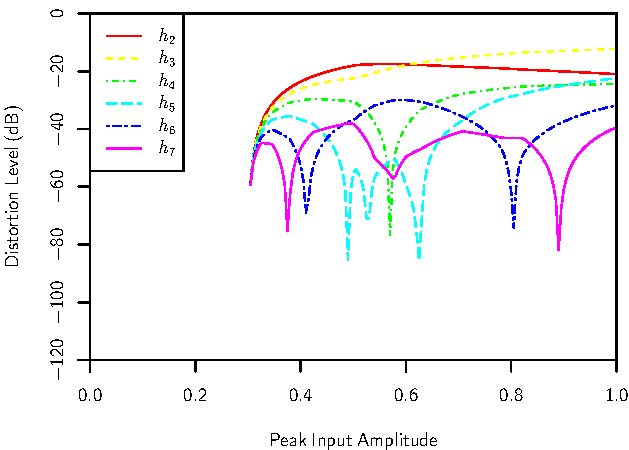
\includegraphics{chapter5/Images/AsymmetricHardClippingHarmonics.pdf}
				\caption{Individual harmonic distortion levels for Equation
					 \ref{eq:AsymmetricHardClipping} with thresholds of -0.3 and 0.5.}
				\label{fig:AsymmetricHardClippingHarmonics}
			\end{figure}

			The amplitudes of the generated harmonics will roll off at differing rates depending on the
			properties of the output signal. The spectrum will roll off at $6(n+1)$dB per octave when
			the $n$\super{th} derivative of the output signal is discontinuous \citep{kraght2000aliasing}.

			Hard clippers introduce discontinuities to the first derivative of a signal and so will introduce
			harmonics whose amplitudes will roll off at 12dB per octave. Signals clipped by Equation
			\ref{eq:SymmetricSoftClipping} are continuous in the first derivative and so produce harmonics
			which roll off at a faster rate. This can be seen in Figure \ref{fig:ClippingSpectra}.

			\begin{figure}[h!]
				\centering
				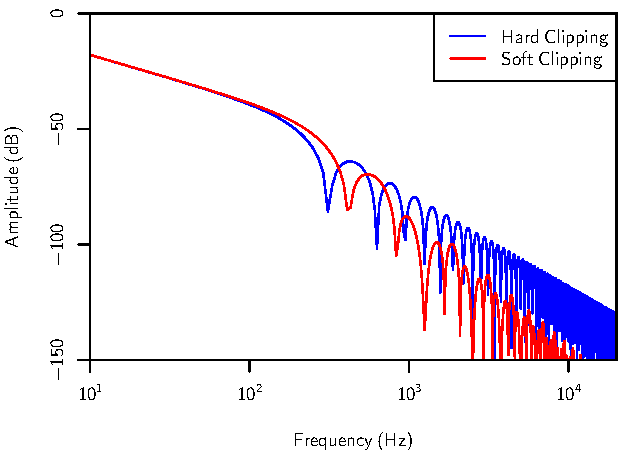
\includegraphics{chapter5/Images/ClippingSpectra.pdf}
				\caption{Spectra of sinusoids clipped using Equations \ref{eq:SymmetricHardClipping} and
			                 \ref{eq:SymmetricSoftClipping}.}
				\label{fig:ClippingSpectra}
			\end{figure}

			The large amount of spectral content introduced by static nonlinearities means they are
			particularly susceptible to aliasing. Through smoothing the characteristic curve of the
			nonlinearity (making the clipper `softer') the amplitudes of generated frequencies will roll of
			more quickly. With lower levels of high order distortion the amplitudes of any aliased components
			will be reduced.

		\subsubsection*{Rectification}
			Full wave rectification can be considered as a static nonlinearity with an even characteristic
			curve, as such it only introduces even order distortion components. The Fourier coefficients of a
			rectified sine wave are shown in Equation \ref{eq:RectificationFourier}.


			\begin{gather}
				c_{n} = \frac{1}{2\pi} \int_{-\pi}^{\pi} \abs{sin(x)}e^{-inx} dx \nonumber \\
				c_{n} = \begin{cases}
					\frac{2}{\pi(1 - n^{2})} & \text{when $n$ is even} \\
					0 & \text{when $n$ is odd}
				\end{cases}
				\label{eq:RectificationFourier}
			\end{gather}

			This represents all even order harmonics rolling off at approximately 12dB per octave.  As with
			other static nonlinearities, rectifiers are susceptible to aliasing. The relatively shallow roll
			off of the distortion components can lead to a considerable amount of energy present in the aliased
			components of the output signal. 

			The output from a half wave rectifier has the same spectrum as that of a full wave rectifier but
			with the content of the original signal included. This can easily be shown by considering how a half
			wave rectified signal can be constructed from the original signal and a full wave rectified signal.
			Where $x[n]$, $x_{f}[n]$ and $x_{h}[n]$ represent the original signal, full wave rectified and half
			waves rectified signals respectively, their relationship can be seen in Equation
			\ref{eq:RectificationRelationship}.

			\begin{equation}
				x_{h}[n] = \frac{1}{2} \left( x_{f}[n] + x[n] \right)
				\label{eq:RectificationRelationship}
			\end{equation}

		\subsubsection*{Integrator}
			Applying Equation \ref{eq:Integrator} to a sine wave produces a signal with Fourier coefficients as
			shown in Equation \ref{eq:IntegratorFourier}.

			\begin{gather}
				c_{n} = \frac{kf_{s}}{2\pi} \left( \int_{0}^{\pi} (1 - cos(x))e^{-inx} dx +
							\int_{\pi}^{2\pi} (3 + cos(x))e^{-inx} dx \right) \nonumber \\
				c_{-1} = - \frac{2ikf_{s}}{\pi} \nonumber \\
				c_{0} = 2kf_{s} \nonumber \\
				c_{1} = \frac{2ikf_{s}}{\pi} \nonumber \\
				c_{n} = \frac{ikf_{s}}{2\pi} \left( \frac{4n^{2} + 2e^{-i\pi n} - 2}{n^{3} - n} \right)
				\label{eq:IntegratorFourier}
			\end{gather}

			This produces all harmonics with amplitudes rolling off at approximately 6dB per octave. This
			shallow roll of make integrators very useful when a large amount of new frequency content is
			desired. Due to the shallow roll off of the distortion component's amplitudes integrators are very
			prone to aliasing.

			While integrators are homogeneous, they are frequency dependant acting as low pass filters. Using
			the same integration constant a high frequency input signal will produce a lower amplitude output
			than a low frequency input. This does not affect the relatives amplitudes of frequencies in the
			output just the overall amplitude of the signal.

		\subsubsection*{Multiplier}
			Nonlinear processing using Equation \ref{eq:Multiplier}, in which the exponent is a positive
			integer, allows for control over the maximum order of distortion generated. The highest frequency
			present among those generated will be equal to the highest frequency in the input signal multiplied
			by the exponent. This facilitates more control over the bandwidth of the generated signal providing
			greater flexibility and minimisation of aliasing.

			If the exponent is allowed to take any positive value, control over the bandwidth of the output
			signal is lost. Non integer exponents cause higher orders of distortion to be generated. Figures
			\ref{fig:CubedSpectra} and \ref{fig:TwoAndAHalfSpectra} show the spectral effects of exponential
			distortion with integer and non-integer exponents. The input signal has a fundamental frequency of
			1kHz and has energy in the first four harmonics.

			\begin{figure}[h!]
				\centering
				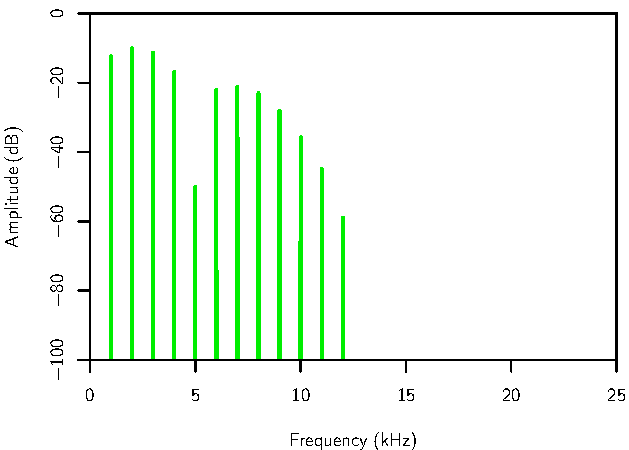
\includegraphics{chapter5/Images/CubedSpectra.pdf}
				\caption{The spectral effects of cubing a signal with energy in its first four harmonics.}
				\label{fig:CubedSpectra}
			\end{figure}

			\begin{figure}[h!]
				\centering
				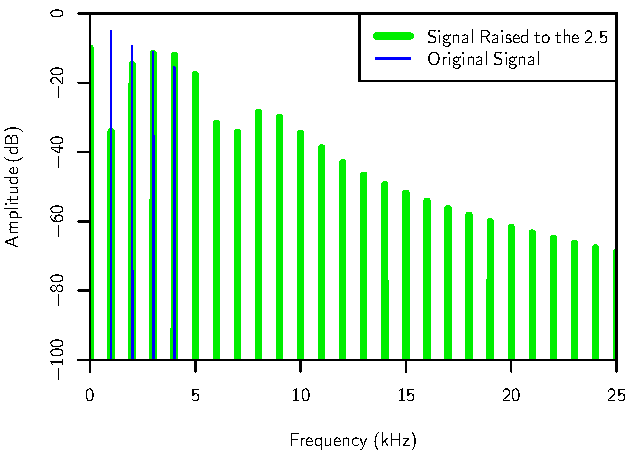
\includegraphics{chapter5/Images/RaisedToTwoAndAHalfSpectra.pdf}
				\caption{The spectral effects of raising a signal with energy in its first four harmonics
					 to the power 2.5.}
				\label{fig:TwoAndAHalfSpectra}
			\end{figure}

			The highest frequency component in the original signal is 4kHz. After cubing the signal the highest
			frequency is three times this (12kHz) as seen in Figure \ref{fig:CubedSpectra}. Figure
			\ref{fig:TwoAndAHalfSpectra} shows that when the exponent is 2.5 higher frequency components are
			introduced. 

		\subsubsection*{SSBA}
			SSBA extends the control provided by multipliers as it constrains the minimum frequency introduced
			as well as the highest. Using Equation \ref{eq:SSB} only the upper sideband (the sum frequencies)
			of the modulation is produced. The highest and lowest frequency components of the output are that
			of the input signal multiplied by the exponent. Between these two frequencies lie all the other
			harmonic and intermodulation components created. This can be seen in figure \ref{fig:SSBA3Spectra},
			which shows the results of applying $3^{rd}$ order SSBA to the signal used in Figures
			\ref{fig:CubedSpectra} and \ref{fig:TwoAndAHalfSpectra}. 			
			
			\begin{figure}[h!]
				\centering
				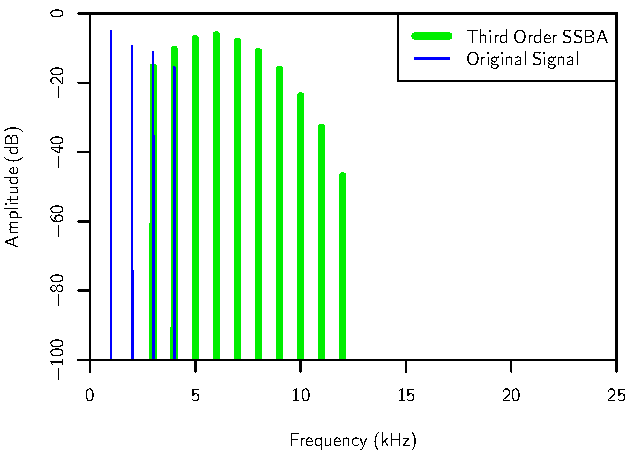
\includegraphics{chapter5/Images/SSBA3Spectra.pdf}
				\caption{The spectral effects of applying third order SSBA to a signal with energy in its 
				         first four harmonics.}
				\label{fig:SSBA3Spectra}
			\end{figure}

			If aliasing does occur it is possible for the aliased frequency to lie outside of this bandwidth.
			The amplitude of aliased frequencies can be greatly reduced through filtering. Applying a low pass
			filter with a cutoff frequency of $\frac{f_{s}}{2h}$ prior to processing will reduce the amplitude
			of any frequency content in the input which will cause aliasing when processed.

		\subsubsection*{IAP}
			In contrast to the SSBA method, the IAP method is homogeneous but provides little control over the
			bandwidth of the output when the input has multiple frequency components. Figure
			\ref{fig:IAP3Spectra} shows the spectral effects of third order IAP processing on the same signal
			used when discussing previous algorithms.

			\begin{figure}[h!]
				\centering
				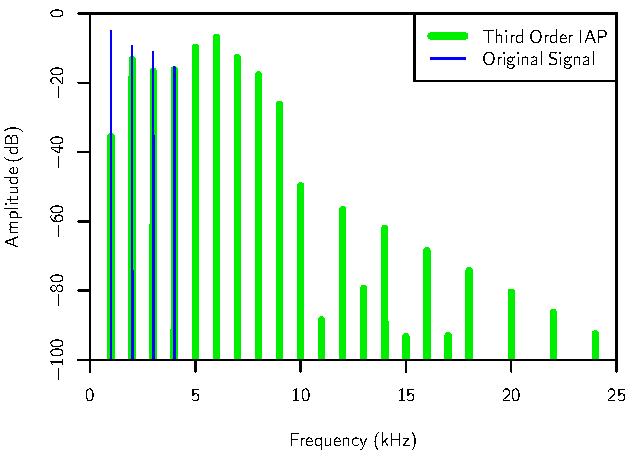
\includegraphics{chapter5/Images/IAP3Spectra.pdf}
				\caption{The spectral effects of applying third order IAP to a signal with energy in its 
				         first four harmonics.}
				\label{fig:IAP3Spectra}
			\end{figure}

			When multiple frequency components are present in the input signal, IAP processing produces energy
			at high order distortion components. As with previous algorithms, it may be necessary to upsample
			the signal before processing to avoid aliasing of these frequencies.

		\subsubsection*{Spectral Replication}
			In spectral replication each frequency component is shifted by the same amount preserving the size
			of the spacings between them. This is useful for harmonic excitation of simple harmonically
			structured signals. Providing the spectrum is shifted by an integer multiple of the fundamental
			frequency any components at harmonic frequencies in the input will remain harmonic frequencies at
			the output. This process avoids the intermodulation distortion inherent to the systems discussed
			previously. 

			Due to every frequency component being shifted by an equal amount the bandwidth of the output is
			equal to that of the input. This predictability allows for easier control of the output spectrum.
			It also provides a simple method for reduction of aliasing. The highest frequency in the output
			will be that of the input plus the shift frequency $f$. Applying a low pass filter, with a cutoff
			frequency of $f_{s} - f$Hz to the input will help minimise the amplitude of any aliased
			frequency components.

		\subsubsection*{Spectral Folding}
			Spectral folding with a factor $k$ results in the lowest $\frac{1}{k}$ of the input spectrum being
			repeated $k$ times in the output spectrum. Every second repetition is a mirror image of the
			original. This effect is shown in Figure \ref{fig:SpectralFolding}. 
			
			\begin{figure}[h!]
				\centering
				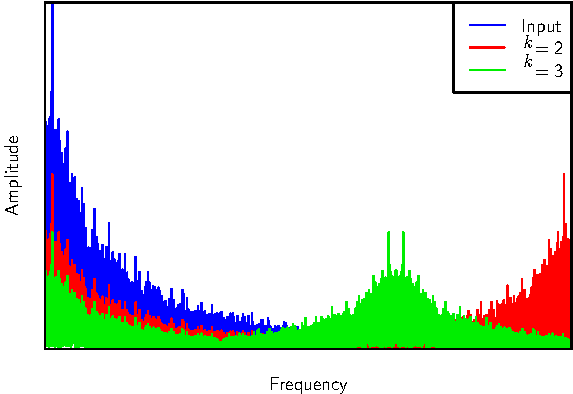
\includegraphics{chapter5/Images/SpectralFoldingSpectrum.pdf}
				\caption{The spectral characteristics of spectral folding.}
				\label{fig:SpectralFolding}
			\end{figure}

			The new frequencies introduced in the output depend on the sampling rate of the signal. Unless
			$\frac{f_{s}}{2k}$ is a harmonic of the input signal, there is little chance that the new
			frequencies will be harmonically related to the input.

			Other than changing the downsampling / upsampling factor, the user is given little control over the
			content of the output spectrum. The bandwidth of the output is not constricted, possibly taking up
			the entirety of the spectrum. Additional filtering is needed to shape the output spectrum as
			desired, increasing the overall complexity of the system.

		\subsubsection*{Spectral Stretching}
			An ideal spectral stretching system would produce the result shown in Figure
			\ref{fig:SpectralStretching}. All frequency components are scaled by the same factor. For
			harmonically structured signals this has the effect of scaling the fundamental frequency.

			The phase vocoder introduces some artefacts during its operation. The process of splitting the
			signal into frames causes spectral leakage. Energy at a given frequency is spread across the nearby
			frequencies. In a signal which only has energy at harmonic frequencies, spectral stretching by an
			integer factor will produce some inharmonic content due to this effect. Spectral leakage can be
			minimised through the use of windowing functions such as the Hamming or Blackman-Harris windows. 

			Ignoring the effect of spectral leakage, the bandwidth of the output signal will be that of the
			input multiplied by the stretching factor. This allows for effective minimisation of aliasing as
			the signal can be low pass filtered before processing as done with single sideband automodulation.
		
		\subsubsection*{STTR}
			The spectral effects of STTR depend on factors of the input signal and the window function and
			step size used. For simple sinusoidal inputs complex output spectra can be generated. For example
			consider the spectral effects of STTR using the window function defined in Equation
			\ref{eq:STTRWindow} (shown in Figure \ref{fig:STTRWindow}).

			\begin{equation}
				w[n] = \begin{cases}
					\cos \left( \frac{4\pi n}{3L} \right) & \text{if $\abs{n} \leq \frac{L}{4} $} \\
					1 - \cos \left( 2\pi \frac{2n - \sgn(n)L}{3L} \right) &
						\text{if $\frac{L}{4} < \abs{n} \leq \frac{L}{2}$} \\
					0 & \text{otherwise}
				\end{cases}
				\label{eq:STTRWindow}
			\end{equation}

			\begin{figure}[h!]
				\centering
				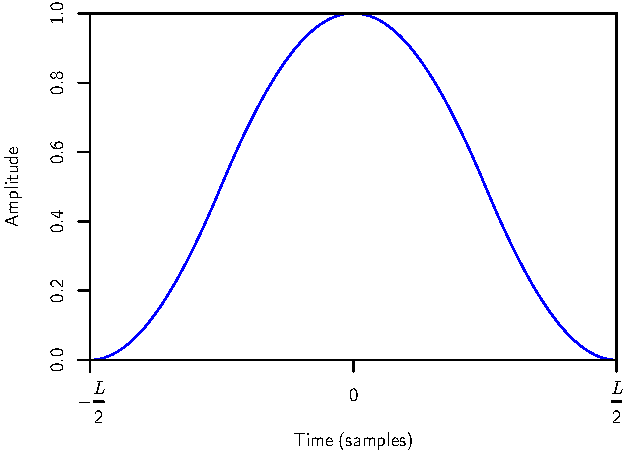
\includegraphics{chapter5/Images/STTRWindow.pdf}
				\caption{The window function defined in Equation \ref{eq:STTRWindow}.}
				\label{fig:STTRWindow}
			\end{figure}

			This window function exhibits constant overlap add for a step size of $\frac{L}{2}$.

			Figure \ref{fig:STTRSpectra} shows the output spectra of STTR, using this window with lengths of
			1ms and 1.5ms, on a 1kHz sinusoid.

			\begin{figure}[h!]
				\centering
				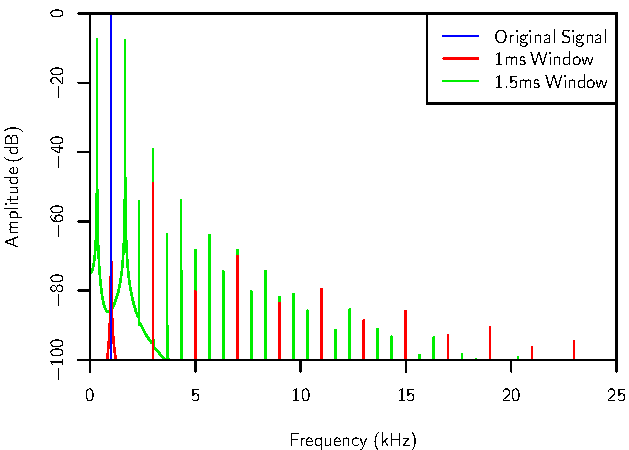
\includegraphics{chapter5/Images/STTRSpectra.pdf}
				\caption{The spectral effects of STTR using the window function defined in Equation
				         \ref{eq:STTRWindow}.}
				\label{fig:STTRSpectra}
			\end{figure}

			The complexity of the output spectrum depends on the relationship of the input frequency and the
			step size used for processing. If the period of the input signal is an integer multiple of the step
			size, it will remain unchanged by the processing. This is evidenced by the output spectrum for 1ms
			window shown in Figure \ref{fig:STTRSpectra}, only odd order harmonics are generated retaining the
			original period of the signal.

			The period of the output signal is the least common multiple of the period of the input signal and
			the step size. This causes the period of a signal to be increased when the period of the input is
			not an integer multiple of the step size. The output spectrum for a 1.5ms window shows this. The
			period of the output becomes 3ms. The lowest frequency in this output is then approximately 333Hz.

			The exact frequencies of the partials in the output are discussed by \citet{kim2014shorttime}. In
			effect they are the intermodulation frequencies of the input frequency and the step frequency (1
			over the step size in seconds). The amplitudes of these partials are influenced by the Fourier
			transform of the window function used. This allows the spectral characteristics of the output to be
			loosely controlled through manipulation of the window function and step size.

			There is no upper bound on the frequency of the output so upsampling may need to be used to
			minimise aliasing.

	\subsection{Temporal Characteristics}
	\label{sec:ExcitationEvaluation-Comparison-TemporalCharacteristics}
		\subsubsection*{Static Nonlinearities}
			As static nonlinearities are memoryless they can not influence the temporal evolution of signals at
			a large scale. There is a possibility to affect the attack and release times of signals slightly
			through increasing the gradient of the low amplitude section characteristic curve. As an extreme
			example consider the infinite peak clipper shown in Equation \ref{eq:InfinitePeakClipper}.

			\begin{equation}
				y[n] = \begin{cases}
					-1 & \text{if $x[n] < 0$} \\
					0 & \text{if $x[n] = 0$} \\
					1 & \text{if $x[n] > 1$}
				\end{cases}
				\label{eq:InfinitePeakClipper}
			\end{equation}
			
			Figure \ref{fig:InfinitePeakClipping} shows a signal, with attack and release sections, before and
			after infinite peak clipping. The original signal rises to its full amplitude over two cycles and
			falls back to silence over the same time. After infinite peak clipping the attack and release have
			become instantaneous.

			\begin{figure}[h!]
				\centering
				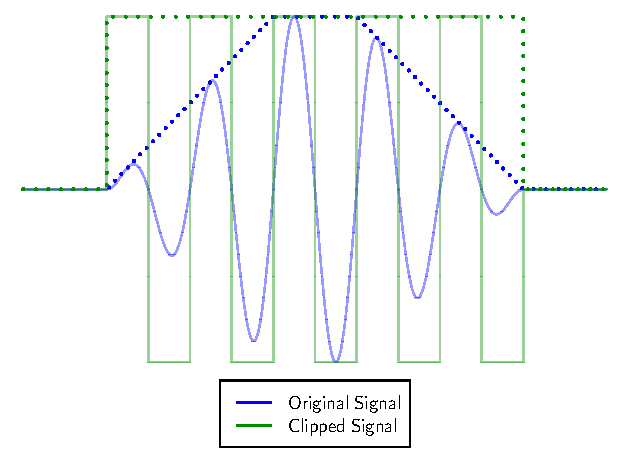
\includegraphics{chapter5/Images/InfinitePeakClipping.pdf}
				\caption{A graph showing a signal before and after infinite peak clipping.}
				\label{fig:InfinitePeakClipping}
			\end{figure}

		\subsubsection*{Rectification}
			Full wave rectifiers have no effect on the temporal characteristics of signals as all the magnitude
			of each sample is preserved. It is possible that a half wave rectifier could change the position of
			the onset of a signal by a small amount. Considering a signal which starts with a negative
			displacement. This first section of the signal would be removed, moving the onset to wherever the
			first positive displacement occurs.
			
		\subsubsection*{Integrator}
			Due to the inherent low pass filtering behaviour of integrators the temporal properties of
			transient signals will be altered. Attacks times will be lengthened by the attenuation of their
			high frequency components. This prevents these methods being used where it is essential that
			transients are preserved. 
			
		\subsubsection*{Multiplier}
			Exponential distortion has a dynamic compression/expansion effect. For exponents greater than 1 the
			dynamics of a signal are expanded, the amplitude difference between low and high amplitude portions
			of the signal is increased. For exponents less that 1 the opposite occurs, compressing the dynamics
			of the signal. Figure \ref{fig:ExponentiationTemporalEffects} show the effects this can have on the
			attack and release portions of signals.

			\begin{figure}[h!]
				\centering
				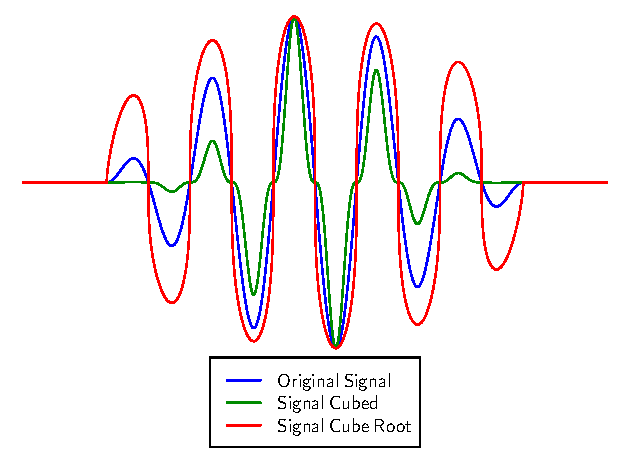
\includegraphics{chapter5/Images/ExponentiationTemporalEffects.pdf}
				\caption{The temporal effects of exponential distortion.}
				\label{fig:ExponentiationTemporalEffects}
			\end{figure}

			While the time taken for the signal to rise to or decay from maximum amplitude is not changed, the
			shape of the amplitude envelope during the attack and release portions is. 

		\subsubsection*{SSBA}
			SSBA has similar temporal effects to a multiplier using an exponent greater that 1. The signal
			undergoes dynamic expansion changing the shape of its attack and release envelopes as shown in
			Figure \ref{fig:SSBATemporalEffects}.

			\begin{figure}[h!]
				\centering
				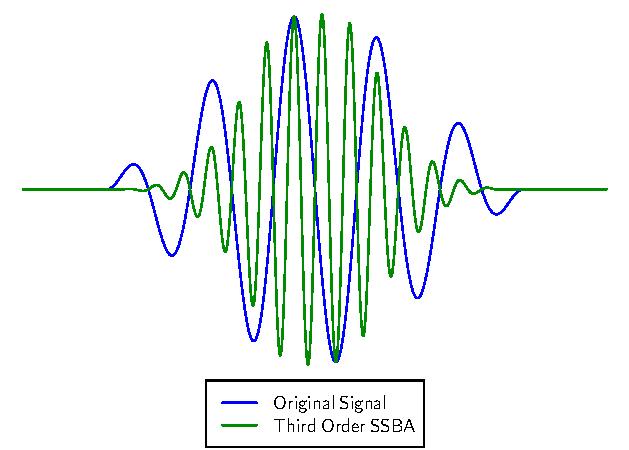
\includegraphics{chapter5/Images/SSBATemporalEffects.pdf}
				\caption{The temporal effects of SSBA.}
				\label{fig:SSBATemporalEffects}
			\end{figure}

			The restricted bandwidth of the SSBA technique's output is also apparent from this graph. The input
			is a sinusoid with a simple amplitude envelope. The output is a sinusoid with 3 times the frequency
			and an amplitude envelope equal to that of the input cubed. This is in contrast to the effect of
			the multiplier shown in Figure \ref{fig:ExponentiationTemporalEffects} where the output signal is
			no longer sinusoidal.

		\subsubsection*{IAP}
			The homogeneity of the system preserves the input signals amplitude envelope. Due to this the
			temporal characteristics of signals are unaffected. This can be seen in Figure
			\ref{fig:IAPTemporalEffects}, it is apparent that the frequency of the sinusoid has been altered
			and its amplitude envelope not.

			\begin{figure}[h!]
				\centering
				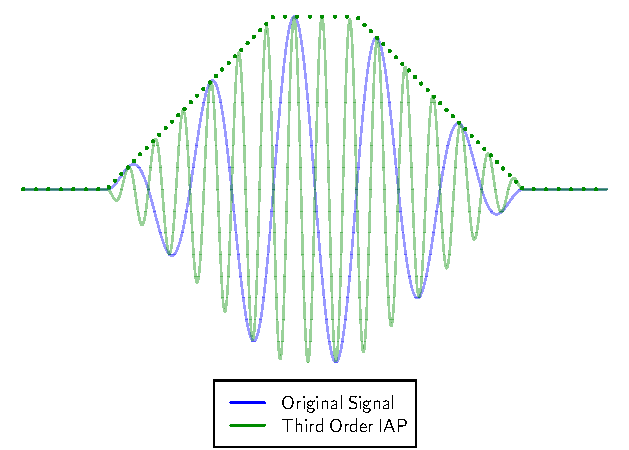
\includegraphics{chapter5/Images/IAPTemporalEffects.pdf}
				\caption{The temporal effects of IAP.}
				\label{fig:IAPTemporalEffects}
			\end{figure}
			
		\subsubsection*{Spectral Replication}
			Spectral replication does not affect the temporal properties of a signal.

		\subsubsection*{Spectral Folding}
			The low pass filter applied as part of the downsampling phase removes the high frequency content
			which contributes to transients in the signal. This has the effect of lengthening attack times
			similar to the effect seen in the Integrator system (Section
			\ref{sec:Excitation-Methods-Integrator}).

		\subsubsection*{Spectral Stretching}
			A simple phase vocoder implementation produces artefacts when processing transients in a signal.
			The phase correction stage before resynthesis can have the effect of softening the attack portion.
			The exact effect had on the transient is not able to be controlled as it depends on where the
			transient lies in the STFT frame. \citet{robel2003a} proposes a method to better process transients
			with a phase vocoder. An algorithm is used to detect the presence of transients in an STFT frame.
			The phase information is then processed differently depending on the position of the transient
			within the frame.

		\subsubsection*{STTR}
			Due to the time reversal STTR can have complicated effects on a signal's amplitude envelope.
			For instance, the attack and release portion of a sound may be switched. While possible, this is
			highly dependent on the window length, step size and content of the input frequency. Controlling
			these aspects for general input signals proves a very difficult task.

	\subsection{Flexibility}
	\label{sec:ExcitationEvaluation-Comparison-Flexibility}
		\subsubsection*{Static Nonlinearities}
			For musical signals static nonlinearities introduce a spectrally rich band of audio. The spectral
			content of which is highly dependent on that of the input signal. The bandwidth of the new set of
			frequencies can be easily controlled through filtering or through the techniques discussed for
			reducing aliasing. This allows for good performance in situations where energy needs to be added to
			a specific area of the spectrum. 

		\subsubsection*{Rectification}
			Rectifiers are useful when large amounts of even order distortion components are required. As with
			other static nonlinearities, the bandwidth of the newly introduced set of frequencies can be
			controlled through filtering to provide more flexibility. 

		\subsubsection*{Integrator}
			Integrators provide an efficient means to add wideband energy to the spectrum of a signal. All
			orders of distortion are generated making this new signal spectrally dense. The bandwidth of the
			new signal can easily be controlled through filtering improving the flexibility.

		\subsubsection*{Multiplier}
			Multipliers offer greater flexibility than the previously discussed excitation methods. Control
			over the orders of distortion introduced allows for finer shaping of a signal's spectrum. The
			output of several multipliers with different exponents can be summed in order to include multiple
			orders of distortion.

			Summing multiplier outputs in this way allows for approximation of other static
			nonlinearities. A low order polynomial expression approximating the desired characteristic curve
			is calculated by linear regression as shown in Figure \ref{fig:ClippingApproximation}. The
			order of the polynomial controls the maximum order of the distortion components.

			\begin{figure}[h!]
				\centering
				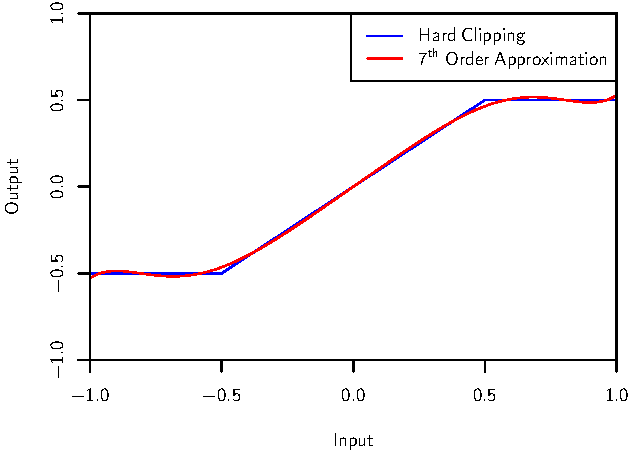
\includegraphics{chapter5/Images/ClippingApproximation.pdf}
				\caption{A 7\super{th} order approximation of hard clipping using linear regression.}
				\label{fig:ClippingApproximation}
			\end{figure}

			Generating characteristic curves in this way reduces the number of aliased frequencies at the cost
			of having to evaluate a more complex polynomial to calculate the output value for each sample. A
			similar approach is undertaken by \cite{fernandez-cid2001distortion} who construct characteristic
			curves from Chebyshev polynomials in order to control the highest frequencies introduced.

		\subsubsection*{Spectral Folding}
			Spectral folding is an efficient method by which to create a dense output spectrum but has many
			downsides.

		\subsubsection*{STTR}
			STTR can be used, much like a static nonlinearity, as a method of generating wide bands of
			high order harmonics. Unlike static nonlinearities however it is possible to generate inharmonic
			partials for a sinusoidal input. The generation of these is dependent on properties of the input
			signal adding further complexity to predicting the effects for arbitrary input signals.

			\citet{kim2015harmonizing} suggest methods through which the output of STTR can be controlled in
			the implementation of a harmonising effect. This effect introduces new tones, at different
			musical intervals, depending on the input frequency. While this is useful as a compositional tool
			it does not provide the uniform response across input signals required for timbral control.

\section{Key Findings}
	\note
	{
		Conclude the chapter.
	}
